\documentclass[compress,12pt]{beamer}

\usetheme{Arguelles}

\usepackage{graphicx}
\usepackage{caption}
\usepackage[spanish,es-noshorthands]{babel}
\usepackage[pages=some]{background}

\usepackage{tikz}
\usepackage{tikz-cd}
\usetikzlibrary{
  babel,
  arrows.meta,
  calc,
  positioning,
  overlay-beamer-styles,
  shadows.blur
}

\usepackage{amsmath,amssymb,latexsym,amscd} 
\usepackage[all,cmtip]{xy}
\usepackage{fancyhdr}
\usepackage{mathalfa}
\usepackage{mathrsfs}
\usepackage{hyperref}
\usepackage{ragged2e}
\usepackage{wasysym}
\usepackage[authoryear]{natbib}

% Colores para la diapositiva Top/Frm
\definecolor{TopBlue}{RGB}{14,73,160}
\definecolor{FrmGreen}{RGB}{15,120,45}
\definecolor{TopLight}{RGB}{235,242,252}
\definecolor{FrmLight}{RGB}{235,248,238}

\pagenumbering{arabic}

\DeclareMathOperator{\op}{op}
\DeclareMathOperator{\pt}{pt}
\DeclareMathOperator{\Sp}{sp}
\DeclareMathOperator{\spec}{spec}
\DeclareMathOperator{\Fit}{Fit}
\DeclareMathOperator{\Pth}{P}
\DeclareMathOperator{\Vrm}{Vrm}
\DeclareMathOperator{\Frm}{Frm}
\DeclareMathOperator{\Top}{Top}
\DeclareMathOperator{\Ord}{Ord}
\DeclareMathOperator{\Obj}{Obj}
\DeclareMathOperator{\Hom}{Hom}

\title{Marcos apilados y fuertemente apilados}
%\subtitle{}
\event{MITAC 2026, BUAP}
\date{\today}
\author{Juan Carlos Monter Cortés \\ Dr. Luis Ángel Zaldívar Corichi}
\institute{Universidad de Guadalajara}
\email{juan.monter2902@alumnos.udg.mx}

%\homepage{www.mywebsite.com}
\github{JCmonter}

\begin{document}


%\frame[plain]{\titlepage}

\begin{frame}[plain]
\titlepage

\vfill
\begin{center}
    \textcolor{white}{\scriptsize Investigación apoyada por SECIHTI-PROYECTO CBF2023-2024-2630}
\end{center}
\end{frame}

\begin{frame}{Contenido}
\tableofcontents
\end{frame}

\section{La noción espacial}
\begin{frame}{Punto de partida}
    \begin{center}
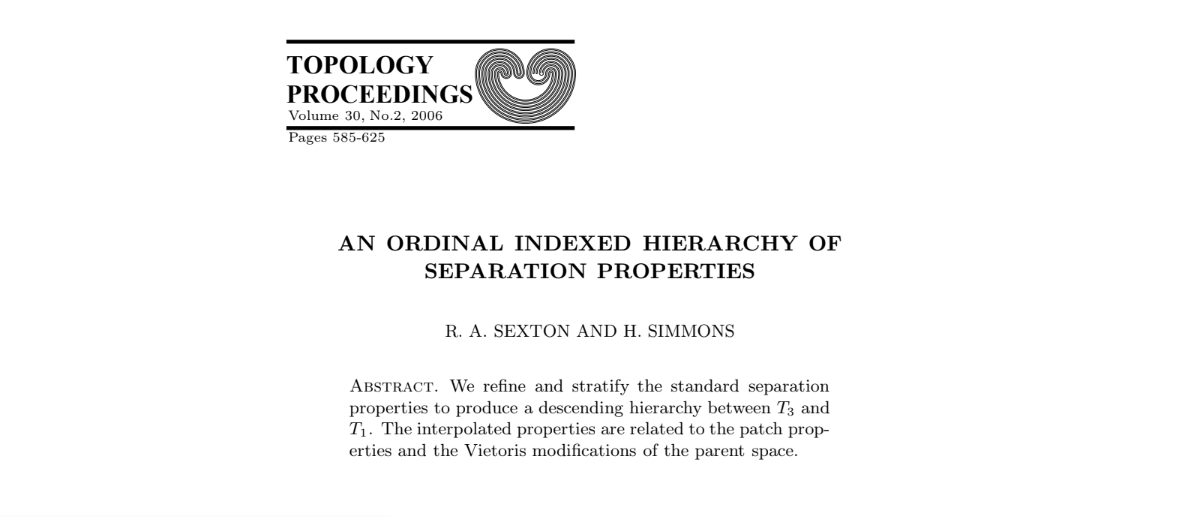
\includegraphics[width=1\textwidth]{Imagenes/Sexton2006.png}
    \end{center}
     {\scriptsize
        R. A. Sexton and H. Simmons,
        \textit{An ordinal indexed hierarchy of separation properties},
        Topology Proceedings \textbf{30} (2006), 585--625.
        }
\end{frame}

\begin{frame}{Derivadas}

Sea \(S\) un espacio topológico.

Un operador
\[
\partial\colon \mathcal{C}S\longrightarrow \mathcal{C}S \qquad 
\]
es una \textbf{derivada} si:
\begin{itemize}
    \item $C\subseteq D\Rightarrow \partial(C)\subseteq \partial(D)$,
    \item $\partial(C)\subseteq C$,
    \item $\partial(C\cup D)=\partial(C)\cup\partial(D)$.
\end{itemize}

Si además
\[
\partial^2=\partial,
\]
decimos que \(\partial\) es una \textbf{derivada idempotente}.
\end{frame}

\begin{frame}{Núcleos espacialmente inducidos}

Sea \(S\) un espacio topológico y \(E\subseteq S\). Consideremos
\[
    [E]\colon\mathcal{O}S\longrightarrow\mathcal{O}S,
    \qquad
    [E](U)=(E\cup U)^\circ.
\]

El operador \([E]\) es un \textbf{núcleo espacialmente inducido}.

\vspace{0.3cm}

Su complemento dual es la derivada idempotente
\[
    \langle E\rangle\colon\mathcal{C}S\longrightarrow\mathcal{C}S, \qquad \langle E\rangle(X)=\overline{(E\cap X)}.
\]

Si $U=X'\in\mathcal{O}S$ (equivalentemente, \(X=U'\)), entonces
\[
    \boxed{
    \langle E\rangle(X)
    =([E](U))'
    =([E](X'))'.
    }
\]
\end{frame}

\begin{frame}{El teorema de Hofmann--Mislove}

Sea \(S\) un espacio topológico. Consideremos
\[
    Q\in\mathcal{Q}S
    \qquad\text{y}\qquad
    \nabla\in(\mathcal{O}S)^\wedge
\]
relacionados mediante el teorema de Hofmann--Mislove:
\[
    \nabla
    =
    \{V\in\mathcal{O}S\mid Q\subseteq V\}.
\]

Para \(X\in\mathcal{C}S\), definimos
\[
    \partial_Q(X)
    =
    \bigwedge_{Q\subseteq V}
    \overline{V\cap X}.
\]

Su complemento dual es el prenúcleo
\[
    f_\nabla(U)
    =
    \bigvee_{Q\subseteq V}
    (V\cup U)^\circ,
    \qquad U\in\mathcal{O}S.
\]

\end{frame}

\begin{frame}{Iteración del prenúcleo}

El operador \(f_\nabla\) es un prenúcleo, pero no es
necesariamente idempotente.

Consideramos sus iteraciones transfinitas:
\[
    f_\nabla^0
    \leq
    f_\nabla
    \leq
    f_\nabla^2
    \leq
    \cdots
    \leq
    f_\nabla^\alpha
    \leq
    \cdots
\]

hasta alcanzar un ordinal para el cual la iteración se estabiliza.

Denotamos por
\[
    \boxed{f_\nabla^\infty}
\]
al núcleo obtenido mediante este proceso.

El operador \(f_\nabla^\infty\) es el
\textbf{fitted nucleus} asociado a \(\nabla\).

\end{frame}

\begin{frame}{Espacios apilados}
\begin{block}{Definición (\cite{sexton2006ordinal}):}
Sea \(S\) un espacio topológico y \(Q\in\mathcal{Q}S\).

\vspace{0.3cm}

Decimos que \(Q\) es \textbf{apilado} si
\[
    \boxed{
        \overline{Q}=\partial_Q^\infty(S)
    }.
\]

Decimos que \(Q\) es \textbf{fuertemente apilado} si
\[
    \boxed{
        \langle Q\rangle=\partial_Q^\infty
    }.
\]

El espacio \(S\) es \textbf{apilado} (resp. \textbf{fuertemente
apilado}) si cada \(Q\in\mathcal{Q}S\) es apilado
(resp. fuertemente apilado).
\end{block}
\end{frame}

\begin{frame}{¿Por qué estudiar espacios apilados?}

Sexton y Simmons prueban las implicaciones
\[
    \text{neat}
    \Longrightarrow
    \text{fuertemente apilado}
    \Longrightarrow
    \text{apilado}.
\]

Además,
\[
    \boxed{
    T_1+\text{apilado}
    \Longrightarrow
    \text{sobrio}.
    }
\]

\end{frame}

\section{La noción en marcos}
\begin{frame}{¿Qué ocurre en marcos?}

En el caso espacial, la noción de apilamiento se construye a partir de

\[
\begin{array}{ccc}
Q\in\mathcal{Q}S
&\longleftrightarrow&
\nabla\in(\mathcal{O}S)^\wedge,
\\[3mm]
\langle Q\rangle
&&
f_\nabla^\infty.
\end{array}
\]

\vspace{0.4cm}

\begin{center}
\Large
¿Cómo trasladar esta construcción a un marco arbitrario \(A\)?
\end{center}

\end{frame}

\begin{frame}{Hofmann--Mislove--Johnstone}

En el caso espacial,
\[
    \nabla\in(\mathcal{O}S)^\wedge
    \quad\longmapsto\quad
    f_\nabla^\infty .
\]

Para un marco arbitrario \(A\), si \(F\in A^\wedge\),
el Teorema de Hofmann--Mislove--Johnstone determina
un intervalo
\[
    \boxed{
        [v_F,w_F]\subseteq NA
    }.
\]

Su extremo inferior
\[
    \boxed{v_F}
\]
es el \textbf{fitted nucleus} asociado a \(F\).

\end{frame}

\begin{frame}{Pares de Hofmann--Mislove}

Consideremos un filtro abierto de Scott
\[
    F\in A^\wedge
\]
y un compacto saturado
\[
    Q\in\mathcal{Q}S.
\]

Cuando \(F\) y \(Q\) están relacionados mediante la
correspondencia de Hofmann--Mislove, diremos que
\[
    \boxed{(F,Q)}
\]
es un \textbf{par HM}.

\vspace{0.4cm}

Estos objetos determinan, respectivamente,
\[
    \boxed{v_F}
    \qquad\text{y}\qquad
    \boxed{\mathcal{U}_*\circ[Q']\circ\mathcal{U}}.
\]

\end{frame}

\begin{frame}{Intervalos de admisibilidad}

Sea \((F,Q)\) un par HM y
\(\nabla=\nabla(Q)\). Si
\[
    k\in[v_\nabla,w_\nabla],
\]
entonces
\[
    \boxed{
    \mathcal{U}_*\circ k\circ\mathcal{U}
    \in[v_F,w_F].
    }
\]

Por tanto, obtenemos una aplicación
\[
    [v_\nabla,w_\nabla]
    \longrightarrow
    [v_F,w_F],
    \qquad
    k\longmapsto
    \mathcal{U}_*\circ k\circ\mathcal{U}.
\]

\end{frame}

\begin{frame}{Comportamiento de los extremos}

La aplicación
\[
    k\longmapsto
    \mathcal{U}_*\circ k\circ\mathcal{U}
\]
no preserva, en general, ambos extremos del intervalo.

\vspace{0.4cm}

Para el extremo inferior,
\[
    \boxed{
    v_F
    \leq
    \mathcal{U}_*\circ v_\nabla\circ\mathcal{U}
    }.
\]

\vspace{0.5cm}

En cambio, para el extremo superior,
\[
    \boxed{
    w_F
    =
    \mathcal{U}_*\circ w_\nabla\circ\mathcal{U}
    }.
\]

\end{frame}

\begin{frame}{El caso \(T_1\)}

Si el espacio \(S\) es \(T_1\), entonces
\[
    [Q']=w_\nabla.
\]

Por tanto,
\[
    w_F
    =
    \mathcal{U}_*\circ w_\nabla\circ\mathcal{U}
    =
    \mathcal{U}_*\circ[Q']\circ\mathcal{U}.
\]

En consecuencia,
\[
    \boxed{
    v_F
    \leq
    \mathcal{U}_*\circ[Q']\circ\mathcal{U}
    =
    w_F.
    }
\]

\end{frame}

\begin{frame}{Marcos apilados}

\begin{block}{Definición:}
Sea \(A\) un marco y \((F,Q)\) un par HM.

Decimos que \(A\) es \textbf{apilado} si
\[
    \boxed{
    v_F(0)
    =
    \bigl(
        \mathcal{U}_*\circ[Q']\circ\mathcal{U}
    \bigr)(0)
    }
\]
para todo par HM \((F,Q)\).

\vspace{0.5cm}

Decimos que \(A\) es \textbf{fuertemente apilado} si
\[
    \boxed{
    v_F
    =
    \mathcal{U}_*\circ[Q']\circ\mathcal{U}
    }
\]
para todo par HM \((F,Q)\).
\end{block}
\end{frame}

\begin{frame}{Del espacio al marco}

\begin{center}
\begin{tabular}{c@{\qquad\qquad}c}
    \textbf{Espacios} & \textbf{Marcos} \\[0.3cm]

    \((\nabla,Q)\) par HM
    &
    \((F,Q)\) par HM
    \\[0.5cm]

    \textbf{Apilado}
    &
    \textbf{Apilado}
    \\[0.2cm]

    \(
        \overline{Q}=\partial_Q^\infty(S)
    \)
    &
    \(
        v_F(0)
        =
        \bigl(
        \mathcal{U}_*\circ[Q']\circ\mathcal{U}
        \bigr)(0)
    \)
    \\[0.7cm]

    \textbf{Fuertemente apilado}
    &
    \textbf{Fuertemente apilado}
    \\[0.2cm]

    \(
        [Q']=f_\nabla^\infty
    \)
    &
    \(
        v_F
        =
        \mathcal{U}_*\circ[Q']\circ\mathcal{U}
    \)
\end{tabular}
\end{center}

\end{frame}

\begin{frame}
\begin{block}{Proposición:}
Las nociones de \textbf{apilado} y
\textbf{fuertemente apilado} son conservativas.
\end{block}

\textbf{Idea de la prueba:} Sea \(A=\mathcal{O}S\) y \((F=\nabla,Q)\) un par HM.

\vspace{0.2cm}

Si \(S\) es \textbf{fuertemente apilado}, entonces
\[
    v_F=[Q']
\iff    \mathcal{U}_*\circ[Q']\circ\mathcal{U}
    =[Q']=v_F.
\]

Si \(S\) es \textbf{apilado}, entonces
\[
    \overline{Q}=\partial_Q^\infty(S)\iff  (\mathcal{U}_*\circ [Q']\circ \mathcal{U})(\emptyset)=(Q')^\circ=v_\nabla(\emptyset) 
\]
\end{frame}

\End

\section*{\textsc{Referencias}}
\begin{frame}[allowframebreaks]
\bibliographystyle{plainnat}
%\bibliographystyle{plain}
%\bibliographystyle{amsalpha}
\bibliography{research2}
\end{frame}

\begin{frame}[plain,standout]
      \centering
      \Huge{\bfseries \smiley¡Muchas gracias!\smiley}
      %In combination with \textit{plain}, \\
      %it makes a nice thank-you slide!
      %\scalebox{4}{\faGithub} \par\bigskip
      %\url{https://github.com/JCmonter/Apuntes/tree/main/Presentaciones} \\
      %\url{https://ctan.org/pkg/beamertheme-arguelles}
\end{frame}
\end{document}